\ifdefined\COMPLETE
\else
    \input{./preambule-sacha-utf8.ltx}
    \begin{document}
\fi

          \vspace*{-1.2cm}       
                 \intitule{Calculs complexes : cours}
                 
\Asavoir{{\large 1) }\underline{Calculs avec plusieurs opérations}}  

\addtokomafont{labelinglabel}{\textnormal}

\begin{labeling}{On effectue }
\item [On effectue ] d'abord les puissances,
\item [] puis les multiplications / les divisions, 
\item [] puis les additions / les soustractions.
\end{labeling}

\Asavoir{\sc Toujours dans cet ordre}, de gauche à droite.

\bigskip 

\Asavoir{{\large 2) }\underline{Calculs avec des parenthèses}}   

\medskip

On effectue les opérations entre les parenthèses dans l'ordre indiqué ci-dessus, puis on effectue les opérations extérieures, dans l'ordre  indiqué ci-dessus.

% \addtokomafont{labelinglabel}{}
\begin{labeling}{Remarques} 
\item[Remarques] $\bullet$ Pour des parenthèses « dans des parenthèses », on effectue les parenthèses « de plus petit niveau » en premier, puis « on remonte ».
\item [] $\bullet$ Un moins devant des parenthèses fait que l'on inverse les signes (cf exemple  {\large \ding{174}}).
\end{labeling} 

                     
%                 \intitule{Calcul complexes} 


\bigskip 

                 \centerline{\intitule{Exemples rédigés de quatre types}}   
\medskip 
   
\Asavoir{{\large 1) }\underline{Calcul avec plusieurs opérations}} 

 
\setbox1=\vtop{ \hsize=5cm \null % null assure l'alignement par le haut 
\begin{tikzpicture}% [every node/.style={anchor=west}]
  \matrix (m) [matrix of math nodes,
row sep=0cm,column sep=0cm,  
% nodes={rectangle, draw},  
%    nodes in empty cells,
column 1/.style={anchor=base east},
column 2/.style={anchor=base west}]
{
 & \dfrac{1}{2}  +  {\methode{\underbrace{\textcolor{black}{\dfrac{3}{5} \times \left(-\dfrac{2}{7}\right)}}}}
   & &  \text{\methode{\hspace{.2cm} La multiplication est prioritaire} } \\    
= & \dfrac{1}{2}\;+\;\left( -\dfrac{6}{35} \right)   \\    
= & |(a)|\dfrac{1}{2} - \dfrac{6}{35} \\  
= & |(b)|\methode{\underbrace{\textcolor{black}{\dfrac{35}{70} - \dfrac{12}{70}}}} \\   
= & \quad \dfrac{23}{70} \\
};   
\node [right = .1 cm of a.east] (c) {} ; 
\draw[color=blue,->,>=latex] (c) to[out=0,in=0]
   node[midway,right]{\hspace*{.5cm}{
   \methode{ \begin{minipage}[c]{.46\linewidth}
      On met au même dénominateur\\
      pour faire la	 soustraction
   \end{minipage}}}
} (b.east);   
\end{tikzpicture}}

\box1
                   
\Asavoir{{\large 2) }\underline{Calcul avec des parenthèses}} 

\begin{tikzpicture}% [scale=.9]
\node  at (2,7)  {$ \dfrac{1}{2} \div \left(\dfrac{3}{4} + \dfrac{5}{3} - \methode{\underbrace{\textcolor{black}{\dfrac{7}{2} \times \dfrac{5}{2}}}}\right)$};
\node at (8,7) {\methode{Dans la parenthèse la multiplication est prioritaire} } ; 
\node at (0,6) {$=$} ; 
\node  at (2,6)  {$ \dfrac{1}{2}   \div  \left(\dfrac{3}{4} + \dfrac{5}{3} - \;\;\; \dfrac{35}{4}\;\;\;\right)$};

\node at (0,5) {$=$} ; 
\node  at (2.1,5) {$ \dfrac{1}{2} \div \left(
\methode{\underbrace{\textcolor{black}{\dfrac{9}{12} + \dfrac{20}{12} }}}
- \dfrac{105}{12}\right)$};
\node at (8,5){
\methode{\begin{minipage}[c]{.46\linewidth}
      On met au même dénominateur\\
      pour faire les additions et les soustractions
   \end{minipage}
}};
\node at (0,3.9) {$=$} ; 
\node  at (2,3.9) {$ \dfrac{1}{2} \div \left(
\methode{\underbrace{\textcolor{black}{\quad \dfrac{29}{12} \quad -  \dfrac{105}{12} }}}
\right)$};
\node at (0,2.8) {$=$} ; 
\node (a) at (1.6,2.8) {$ \dfrac{1}{2} \div \qquad \left(-\dfrac{76}{12} \right)$};
\node at (0,1.7) {$=$} ; 
\node (b) at (1.25,1.7) {$ \dfrac{1}{2} \times \left(-\dfrac{12}{76} \right)$};
\draw[color=blue,->,>=latex] (a) to[out=0,in=0]
node[midway,right]{ $\qquad$ \methode{\begin{minipage}[c]{.46\linewidth}
      On transforme en multiplication\\
      par l'inverse
   \end{minipage}
}} (b); 
\node at (0,.7) {$=$} ; 
\node  at (1.25,.7) (c) {$ \dfrac{1}{2} \times  \left(-\dfrac{3}{19} \right)$};
\draw[color=blue,->,>=latex] (b.south east) to[out=0,in=0]
node[midway,right]{ $\qquad$ \methode{\begin{minipage}[c]{.46\linewidth}
      On simplifie 
   \end{minipage}
}} (c); 

\node at (0,-.3) {$=$} ; 
\node  at (.6,-.3) {$ - \dfrac{3}{38} $};
\end{tikzpicture}    

\newpage

\Asavoir{{\large 3) }\underline{Parenthèses imbriquées / Signe {\Large \bf - } devant des parenthèses} }

\begin{tikzpicture}% [every node/.style={anchor=west}]
  \matrix (n) [matrix of math nodes,
row sep=0cm,column sep=0cm,  
% nodes={rectangle, draw},  
%    nodes in empty cells,
% column 1/.style={anchor=base east},
column 2/.style={anchor=base west},
column 3/.style={anchor=base west}
]{
& 7 -  \Bigl( 5 \times 8 -6 -\bigl( 3 \times 7 +4 -6 \times  \textcolor{blue}{\underbrace{\textcolor{black}{(-9 +1}}_{-8}})\bigr)\Bigr) \\
= & 7 - \Bigl(  5 \times 8 -6 -\bigl( 3 \times 7 + 4  - \textcolor{blue}{\underbrace{\textcolor{black}{6 \times (-8}}_{-48}})\bigr)\Bigr) \\
= & |(a)| 7 - \Bigl(  5 \times 8 -6 -\bigl(\textcolor{blue}{\underbrace{3\times 7}
_{21}} +4   \textcolor{blue}{\underbrace{\textcolor{black}{-(-48)}}_{+48}}\bigr)\Bigr) \\
 \hbox to .1cm {} & \\
= & |(b)| 7 - \bigl(  5 \times 8 -6 - \textcolor{blue}{\underbrace{\textcolor{black}{(21 + 4 +48 }}_{73}})\bigr) \\
= & 7 - ( \textcolor{blue}{\underbrace{\textcolor{black}{ 5 \times 8}}} -6 - 73) % \hspace*{2.65cm}
& \text{\methode {Multiplication prioritaire}}\\
= & 7 - (\textcolor{blue}{\underbrace{\textcolor{black}{40 -6 -73 )}}} \\
= & |(l)|7 \textcolor{blue}{\underbrace{\textcolor{black}{-(-}}} 39) &  % \hspace*{4cm}
\text{\methode{\parbox{6cm}{Un « - » devant une parenthèse\\$\Longrightarrow$ on change le signe }}}\\
= & |(m)| 7 + 39 \\
= & 46 \\
} ; 
\node [below right = .2cm and 0.1cm of a.center] (e) {} ; 
\node [above right = 0.1cm and 0.3cm of b.center] (f) {} ; 
\draw[color=blue,->,>=latex] (e) to[out=-80,in=80] node[midway,right] {}  (f) ;  
\node [below right = .2cm and 1.6cm of a.center] (g) {} ;  % {\textcolor{red}{$\bullet$}} ;  
\node [above right = 0.1cm and 1.6cm of b.center] (h) {} ; 
\draw[color=blue,->,>=latex] (g) to[out=-110,in=80] node[midway,right] {}  (h) ;  
\draw[color=blue,->,>=latex] (a) to[out=5,in=5] node[midway,right] {\hspace*{1cm}\parbox{3.5cm}{Un « - » devant une\\ $\;\;$parenthèse\\on change le signe }}  (b) ;       
\draw[color=blue,->,>=latex] (l.east) to[out=5,in=5] node[midway,right] {}  (m.east) ;   
\end{tikzpicture}

\bigskip 

\Asavoir{{\large 4) }\underline{Avec de inconnues \ldots} }

\begin{tikzpicture}% [every node/.style={anchor=west}]
  \matrix (n) [matrix of math nodes,
row sep=0cm,column sep=0cm,  
% nodes={rectangle, draw},  
%    nodes in empty cells,
% column 1/.style={anchor=base east},
column 2/.style={anchor=base west}
]{
& 6 + 3x - \bigl( 7x +8 \textcolor{blue}{\underbrace{\textcolor{black}{- (-}}} x -9)\big)  \hspace*{2.2cm}\text{\methode{\parbox{6cm}{Un « - » devant une parenthèse\\$\Longrightarrow$ on change le signe }}}\\
= & |(a)| 6 + 3x - ( 7x +8 + x +9) \\
= &  |(b)| 6 + 3x - ( 8x +17) \\
 \hbox to .1cm {} & \\
= &  |(c)| 6 + 3x -  8x - 17 \\
 \hbox to .1cm {} & \\
= &  |(d)| -5x -11 \\
} ;  
\node [right = 4cm of a.west] (e) {} ; 
\node [right = 3.8cm of b.west] (f) {} ; 
\draw[color=blue,->,>=latex] (e) to[out=0,in=0] node[midway,right] {\hspace*{1.9cm} On calcule...}  (f) ;   
\node [right = 4cm of b.west] (g) {} ; 
\node [right = 3.8cm of c.west] (h) {} ; 
\draw[color=blue,->,>=latex] (g) to[out=0,in=0] node[midway,right] {\hspace{1.8cm} Un « - » devant une parenthèse $\Longrightarrow$ on change le signe }  (h) ;  
\node [right = 4cm of c.west] (i) {} ; 
\node [right = 3.8cm of d.west] (j) {} ; 
\draw[color=blue,->,>=latex] (i) to[out=0,in=0] node[midway,right] {\hspace*{1.9cm} On calcule...}  (j) ;      
\end{tikzpicture}



\ifdefined\COMPLETE
\else
    \end{document}
\fi